\documentclass[twoside,final]{hcmut-report}
\usepackage{codespace}
\usepackage{babel}[vietnamese]
\usepackage{fancyvrb}
% Encodings
\usepackage{gensymb,textcomp}
\usepackage{a4wide,amssymb,epsfig,latexsym,multicol,array,hhline,fancyhdr}
\usepackage{booktabs}
\usepackage{listings}
\usepackage{amsmath}
\usepackage{lastpage}
\usepackage[lined,boxed,commentsnumbered]{algorithm2e}
\usepackage{enumerate}
\usepackage{color}
\usepackage{graphicx}			
\newtheorem{theorem}{Theorem}				% Standard graphics package
\usepackage{array}
\usepackage{tabularx, caption}
\usepackage{multirow}
\usepackage[framemethod=tikz]{mdframed}% For highlighting paragraph backgrounds
\usepackage{multicol}
\usepackage{rotating}
\usepackage{graphics}
\usepackage{geometry}
\usepackage{setspace}
\usepackage{epsfig}
\usepackage{xcolor}
\usepackage{algorithm}
\usepackage{algorithmic}
\usepackage{tikz}
\usepackage{listings}
\usetikzlibrary{arrows,snakes,backgrounds}
\usepackage{hyperref}
\geometry{ a4paper,total={170mm,250mm},left=20mm, top=20mm}

% Better tables
% Wide tables go to https://tex.stackexchange.com/q/332902
\usepackage{array,longtable,multicol,multirow,siunitx,tabularx}

% Better enum
\usepackage{enumitem}

% Graphics
\usepackage{caption,float}

% Add options for figures, like max width, framing, etc.
\usepackage[export]{adjustbox}

% References
% Use \Cref{} instead of \ref{}
\usepackage[nameinlink]{cleveref}

\usepackage{mwe}
\definecolor{codegreen}{rgb}{0,0.6,0}
\definecolor{codegray}{rgb}{0.5,0.5,0.5}
\definecolor{codepurple}{rgb}{0.58,0,0.82}
\definecolor{backcolour}{rgb}{0.95,0.95,0.92}

\lstdefinestyle{mystyle}{
    backgroundcolor=\color{backcolour},   
    commentstyle=\color{codegreen},
    keywordstyle=\color{magenta},
    numberstyle=\tiny\color{codegray},
    stringstyle=\color{codepurple},
    basicstyle=\ttfamily\footnotesize,
    breakatwhitespace=false,         
    breaklines=true,                 
    captionpos=b,                    
    keepspaces=true,                 
    numbers=left,                    
    numbersep=5pt,                  
    showspaces=false,                
    showstringspaces=false,
    showtabs=false,                  
    tabsize=2
}

% Configurations
\coursename{Advanced Programming (CO2039)}
\reporttype{Large Assignment 232}
\title{Functional Programming in Python}
\advisor{& PhD. Trương Tuấn Anh &}
\stuname{%
  & Nguyễn Tiến Khang \textbf{2252304} 
}



\AtBeginDocument{\counterwithin{lstlisting}{section}}

\begin{document}
\coverpage%


\tableofcontents
\listoffigures
\listoftables
%\lstlistoflistings{}
\pagebreak
\section{Preface}
\hspace*{1mm} {In this report, we'll go in-depth on how Python utilizes the functional programming paradigm, as well as detailing its mechanism, features and applying them through some example problems. Afterwards, we'll do some Empirical and Sensitivity analysis do determine its core strengths and weaknesses, such as its runtime, complexity, flexibility some used for solving problems. Finally, to conclude this report, we'll compare Python to other interpreted and compiled languages with regard to their functional capacbilities, more specifically JavaScripts, C++, and examining it compared to another pure functional programming language Scala. After this report, we'll be more proficient on applying the FP paradigm on Python, and thus giving us a more concise and dynamic view on functional programming as a whole!}\\
\hspace*{6.5mm} I would like to express my endless gratitude to Doctor Trương Tuấn Anh, my instructor for Advanced Programming (CO2039), for letting us enjoy a comprehensive 


\section{Introduction}
\hspace*{4mm} In recent years, Functional Programming has proven its strength and usefulness in many different fields of Computer Science and Information Technology. Though esoteric and difficult to approach at first, its concise, mathematical and declarative style of programming has cemented its place in the software world, which such applications as Reactjs, Blaze and Haxl of Facebook (their primary front-end infrastructure which runs on Haskell),  Scalding for Twitter (a Scala library used for data processing at Twitter)...  
\begin{figure}[ht]
\centering
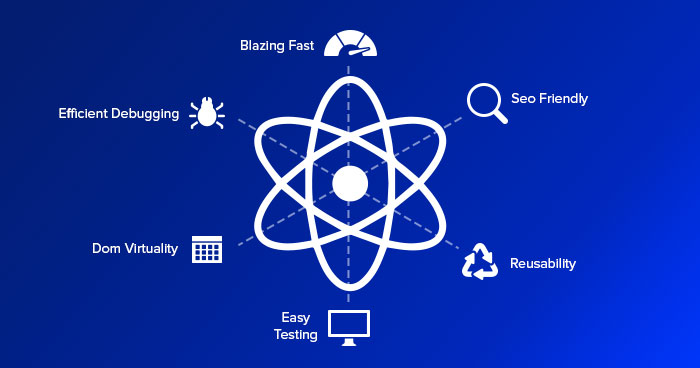
\includegraphics[width=0.5\textwidth]{graphics/reactjs.jpeg}
\caption{In Reactjs, Functional components are usually preferred in development}

\end{figure}

Overall, it has gotten  its place in the world of Computer Science. However, as much as we spend our time diving into the world pure functional languages, it's also important to note that in many high-level, modern, general-purpose languages out there, they still offer a vast amount of functional-based features for developers to explore. Thus, in this report, we've decided to empirically research the in-depth functional aspects of one of the most popular programming languages in the world, \textbf{Python}. Due to its everlasting dominance in a variety of industries and academic fields, there's no question that the first option the most developers and scientists out there would choose is none other than Python itself. Thus, it's a foregone conclusion that one should choose Python as a gentle but thorough introduction to a brand new paradigm.
\\
\hspace*{4mm} One may ask: But how do we proceed with this paradigm shift? What is the effective way to study Python and its "lambda-calculus" ways? 



\section{A Brief History of Python}
\subsection{How Python Was Conceived: The Story Of Guido Van Rossum}
\hspace*{3mm}Although the exact chronology of Python is not very well-documented, modern programmers and enthusiasts still have a wealth of access into how Python came to be.\\
\hspace*{3mm} Python was invented by a Dutch Programmer named \textbf{Guido Van Rossum}. Born in 1956, Rossum was a Mathematics and Computer Science graduate at the University of Amsterdam. A talented and eccentric computer programmer by trait, he first conjured up the idea of Python at around December 1989. According to Rossum, he "had been looking for a 'hobby' programming project that would keep (him) occupied during the week around Christmas."\footnote{Guido Van Rossum - Foreword for "Programming Python" (1st ed.)  - https://www.python.org/doc/essays/foreword/}.  
\begin{figure}[ht]
\centering
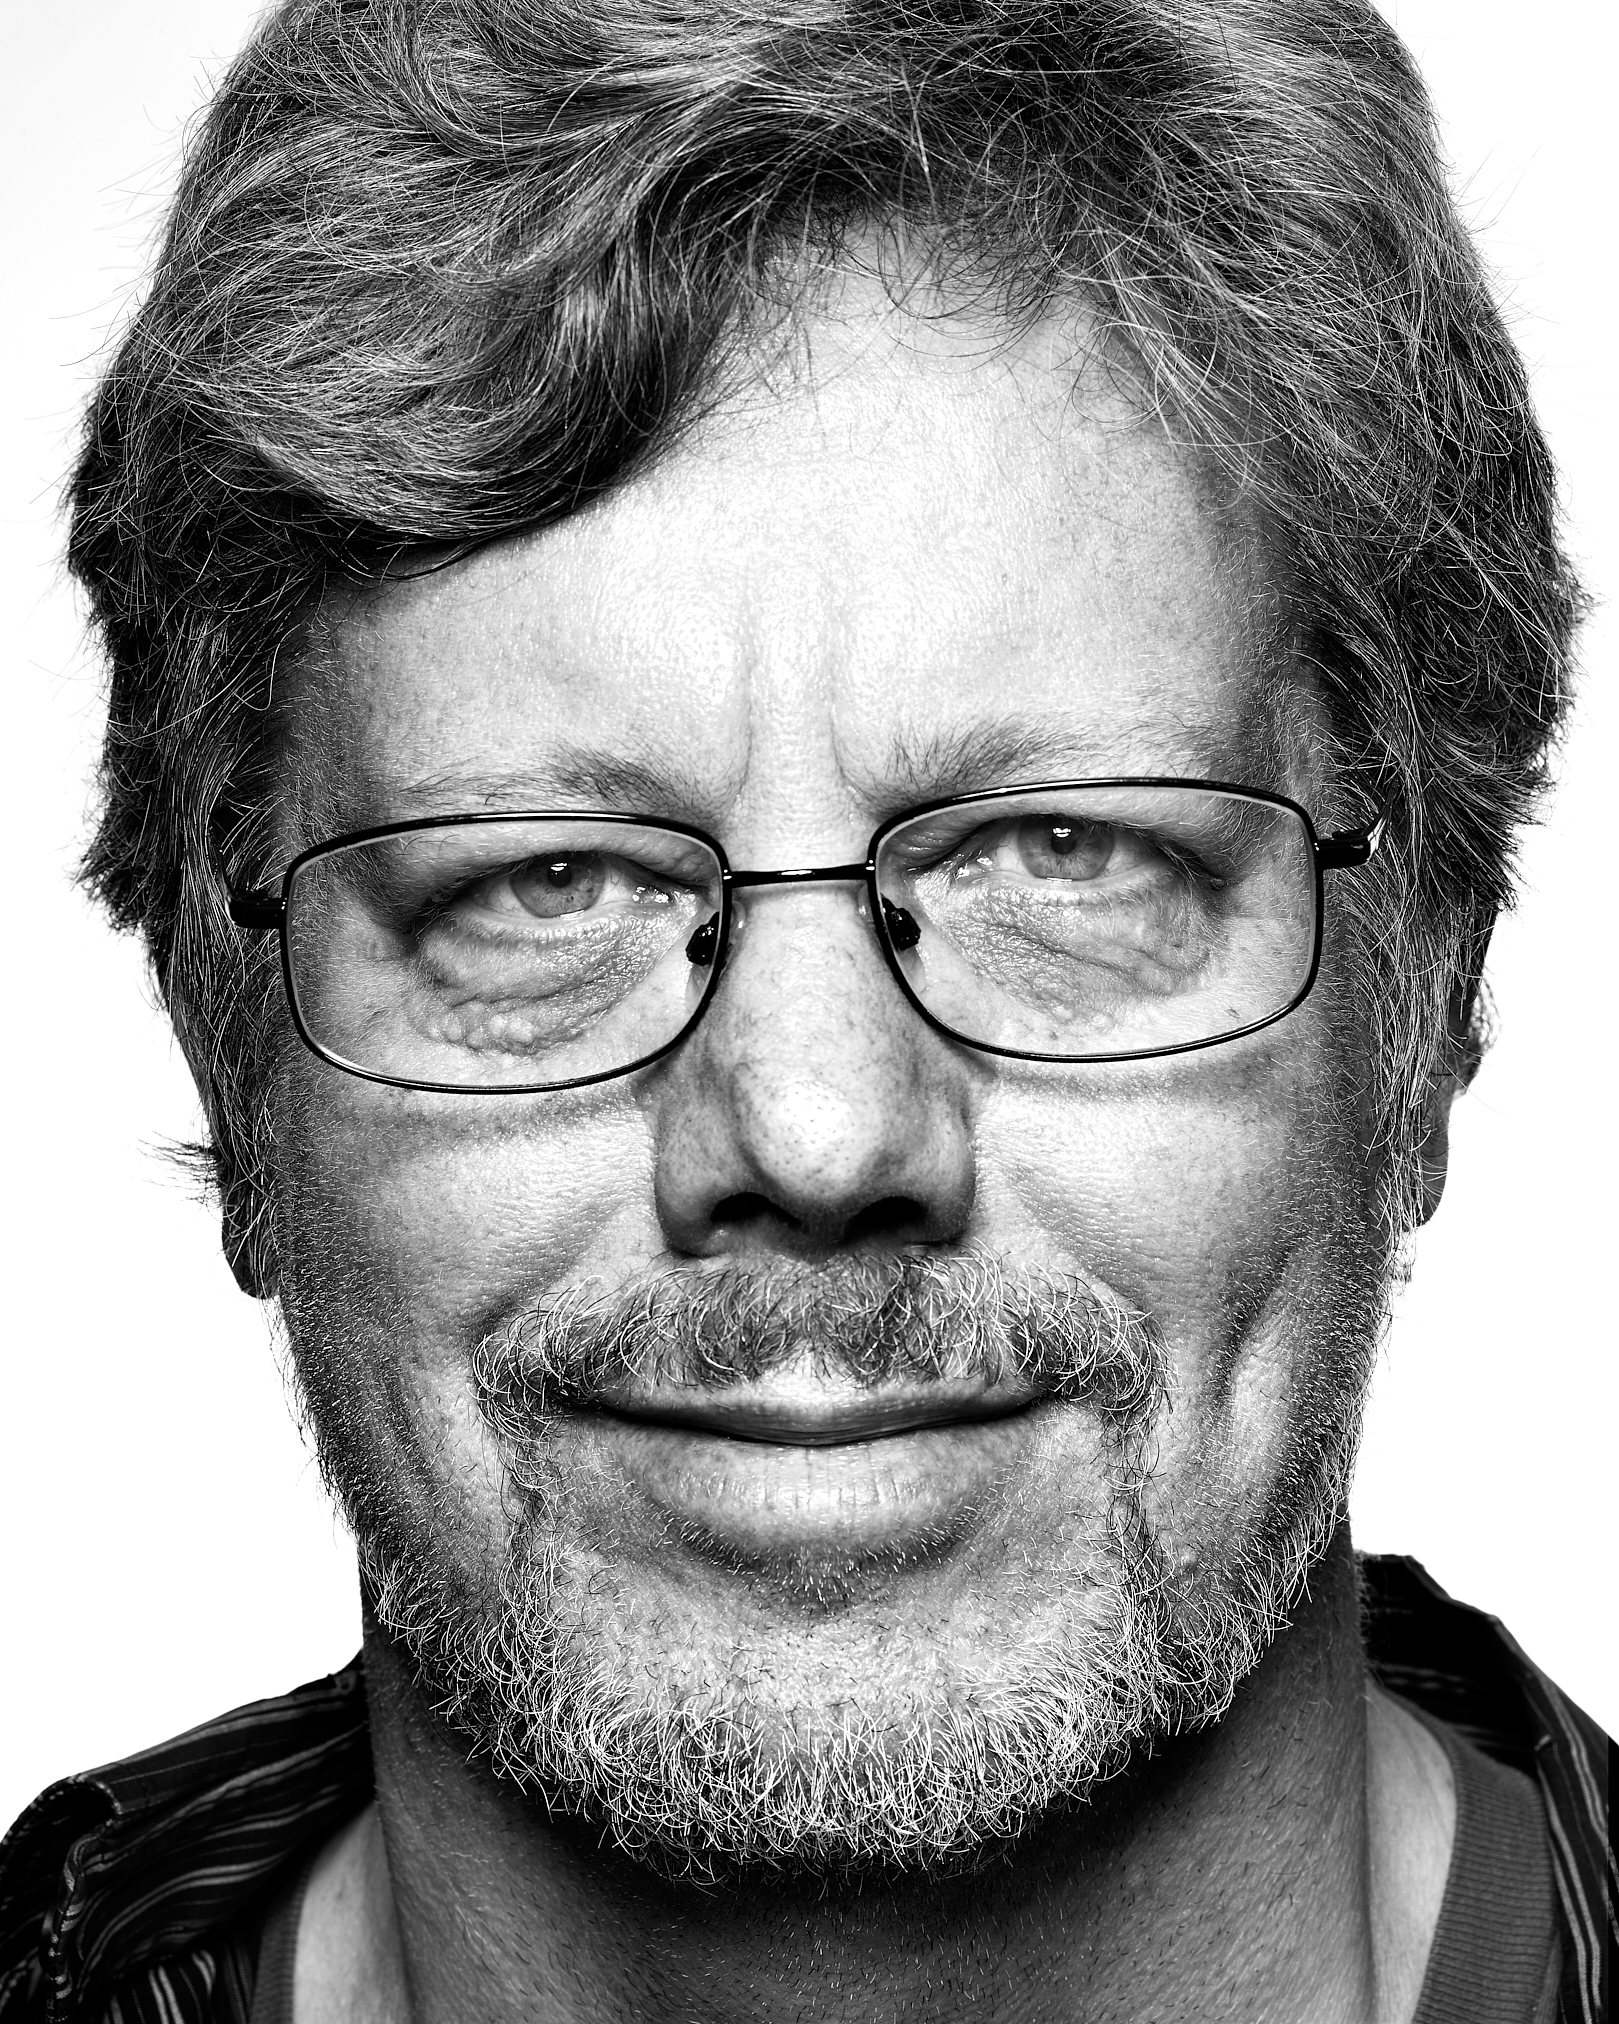
\includegraphics[width=0.35\textwidth]{graphics/rossum.jpeg}
\caption{The Father of Python}

\end{figure}
To put things into context, at the time Rossum was developing system utilities for a microkernel-based distributed system, and of course the work has to be done in C (for low-level design). Due to the primitive syntax of the C language, it was tedious and laborious for him to test out features, functions for the system. Every time he needs to simply test out a procedure, typing out the correct structure of the code is quite a headache. And then, he questioned to himself: "how useful would it be to create a language to help him complete his work faster?". Here's where the very idea of a scripting language comes in. He wanted a readable (like ABC english), high-level language that would greatly reduce the arduousness of typing verbose languages. Though the syntax may be wrapped in layers of abstraction, it's much more preferred when accomplishing quick tasks and simple testing. Moreover, he also wanted to create a language that would appeal somewhat to Unix and C hackers. And with a view to do so, he spent the rest of that Christmas developing what we now called: \textbf{Python 1.0}.

\begin{figure}[ht]
\centering
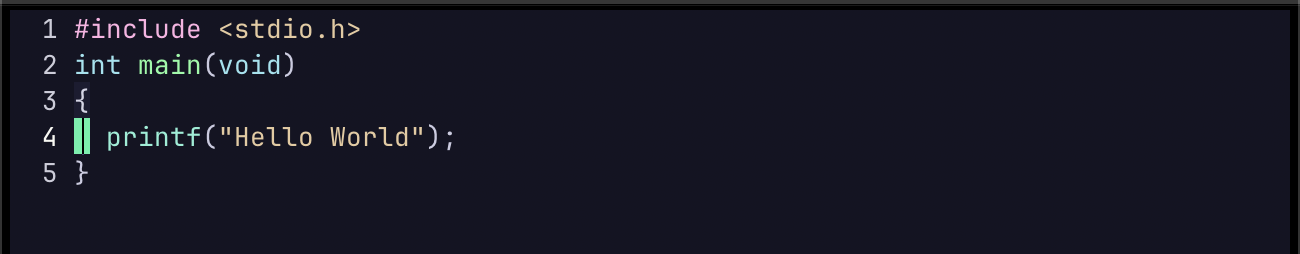
\includegraphics[width=\textwidth]{graphics/c_program.png}
\caption{C programs can be too verbose for simple tasks}
\end{figure}

\hspace*{3mm} With respect to the name, it's a massive misconception that he based it on the animal python, but actually Guido Van Rossum is a huge fan of the renowned English comedy group Monty Python, and decided to choose the group's last name for the project (since he was in an irreverent mood). 
The philosophy of Python can be summed up in "The Zen of Python"\footnote{The Zen of Python - https://peps.python.org/pep-0020/}, which can be called in any Python program through the simple command "import this":

\begin{center}
\begin{BVerbatim}
Beautiful is better than ugly.
Explicit is better than implicit.
Simple is better than complex.
Complex is better than complicated.
Flat is better than nested.
Sparse is better than dense.
Readability counts.
Special cases aren't special enough to break the rules.
Although practicality beats purity.
Errors should never pass silently.
Unless explicitly silenced.
In the face of ambiguity, refuse the temptation to guess.
There should be one-- and preferably only one --obvious way to do it.
Although that way may not be obvious at first unless you're Dutch.
Now is better than never.
Although never is often better than *right* now.
If the implementation is hard to explain, it's a bad idea.
If the implementation is easy to explain, it may be a good idea.
Namespaces are one honking great idea -- let's do more of those!


\end{BVerbatim}
\end{center}
The philosophical ideas of this 19-line manifesto will be discussed in the next section. But it's vital to understand that Python relies on 3 core principles:
\begin{itemize}
\item Readability: the driving force of Rossum's philosophy for Python. It's embedded into the DNA of the language, the central theme of Python that will become crystal clear as we progress into the functional aspects of it.
\item Simplicity: the very concept of Python lies in the scripting nature of it, simple for minuscule tasks.
\item Maintainability: the tenet of Python's philosophy. with a focus on clean code practices encourages developers to write code that is self-explanatory, reducing the potential for bugs and a default, united formatting practice to avoid convolution of formatting styles.


\end{itemize}
\hspace*{3mm} All three principles above are the cornerstone of Python design and "Pythonic" coding. Before embarking on designing Python, Rossum himself already has experience in programming-language design, with ABC and Modula-3 widely regarded as the precursor to Python, with very similar ideas that became inspirations for Python such as Generics, Modularity, OOP,...  With all the background info in mind, how was Python able to enter the world of Computer Programming specifically?

\subsection{The Birth Of A Programming Language: Python }
Although it's muddy what exactly was the date of birth of this language, most have agreed (including Rossum himself) that Python 0.9.0 (the very first version) was released around February 1991. Guido himself published the source code of the Python interpreter to alt.source, a Usenet group for open-source code. Thus began the dynamic story of Python, and open-sourcing helped Python succeed.\\
\hspace*{3mm} Inspired largely by the last language ABC, Python 0.9.0 take the best from ABC and fix the rest. This first Python release had the following essential and modern features:
\begin{itemize}
\item Classes with inheritance exception handling
\item Functions
\item Modules
\item Core data types like list, dict, and str

\end{itemize}
While not popular and hadn't enter the public zeitgeist, this historic moment for Python has certainly made history with many Python lovers around the world. 

\begin{figure}[ht]
\centering
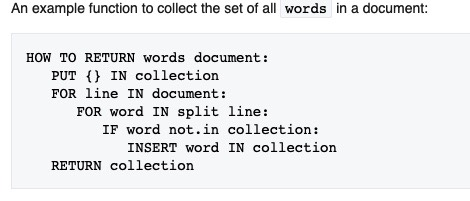
\includegraphics[width=0.8\textwidth]{graphics/ABC.jpeg}
\caption{Snippets of ABC}
\end{figure}
The next major event in Python's lifetime would prove to be a significant one

\subsection{Stepping Into The Spotlight: Python 1.0}
\hspace*{3mm} January 1994, a month to remember, the second version of Python just dropped, ironically named Python 1.0. This is when Python has formed into what's its now known and loved by many. All the central features had been assembled and integrated into the language, including and not limited to lambda, map, filter, complex numbers and other types, The extended library,... All of those features are resemblance of modern programming languages, which add to the groundbreaking work of Guido Van Rossum himself. His brilliance and Python's modernity caught the attention of The National Institute of Standards And Technology in U.S, and they invited him to be an expert and help them learning this new technology. Through his job in the NIST that he had the opportunity to lead workshops, hold conferences and proceedings and generally spread knowledge surrounding Python, attracting various contributors in the Computer world. Eventually, he obtained a position at CNRI (Corporation for National Research Initiatives) and subsequently created a team of Pythonistas and release the future version of the language, as well as created an official website and a mailing list.
\\
\hspace*{3mm} The next major Python update, which he accumulated through previous ventures, would garner Python the status it has today.

\subsection{Becoming Mainstream: Python 2.0}
\hspace*{3mm}In Octorber 16 2000, the programming world not only greeted a new millennium but also was introduced to Python 2.0. What further changes that Python 2.0 entailed? A lot, and this was when Python truly became the norm and captured the minds and hearts of many programmers and scientists around the globe. Python 2.0 (and by extension Python 2.x) introduced numerous improvements and new features, making it a powerful and versatile programming language, essentially enhancing and nurturing what Python 1.0 was best at. Some new features include and not limited to:

\begin{itemize}
\item List comprehension
\item Cycle-detecting garbage collector
\item Support for Unicode
\item Unification of data types and classes
\item A cornucopia of bug fixes
\item Similarity to Haskell

\end{itemize}
And a whole lot more\\

\begin{figure}[ht]
\centering
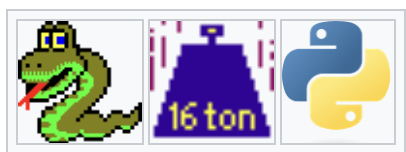
\includegraphics[width=\textwidth]{graphics/logo}
\caption{Evolution of the Python logo\\ From the Windows (left),  Machintosh (center), and from version 2.5 onwards (right)}
\end{figure}

Thanks to Rossum's prior popularity, the update helped Python surged in popularity and cemented its place amongst other programming languages. In the next few years of the 2000s, various modifications and updates to Python would integrated many features that would complete the experience, such as:
\begin{itemize}

\item Python 2.1: A few licensing updates and minor changes (like Statically Nested Scopes)\footnote{PEP 227 – Statically Nested Scopes - https://peps.python.org/pep-0227/}
\item Python 2.2: Unification of Python's type system and the introduction of generators\footnote{Python 2.2 - https://www.python.org/download/releases/2.2/}
\item Python 2.5: Introducing the \textbf{with} statement\footnote{Python 2.5 - https://www.python.org/download/releases/2.5/}

\end{itemize}

\hspace*{3mm} The Python Software Foundation (PSF) played a crucial role in supporting the Python community and facilitating its growth during the 2.x era, since they provide aid in resources, guidance, financial support and advice for the development team. But without community engagement, Python 2.x would never have been as successful as it became. Python remains to this day one of the most active FOSS (free and open-source software) community in the world. Developers, enthusiasts, and experts came together through forums, mailing lists, conferences, and online platforms to discuss Python-related topics and exchange ideas. On the web, users would exchange experience, code, projects, collaboration, APIs and many many other things, in part helping to nurture the growth of the language. The corpus amount of books and references available for Python is a testament how popular this language has become.This vibrant community facilitated the spread of Python's usage, created an environment for learning, and provided support to developers at all levels of expertise. The era of Python 2.x marked a period of consolidation and community growth. Python's increasing popularity among developers was driven by its simplicity, readability, and powerful features. The community-driven development process, fueled by Python Enhancement Proposals (PEPs) and supported by the Python Software Foundation (PSF), ensured that Python evolved based on the needs and feedback of its users. 

\begin{figure}[ht]
\centering
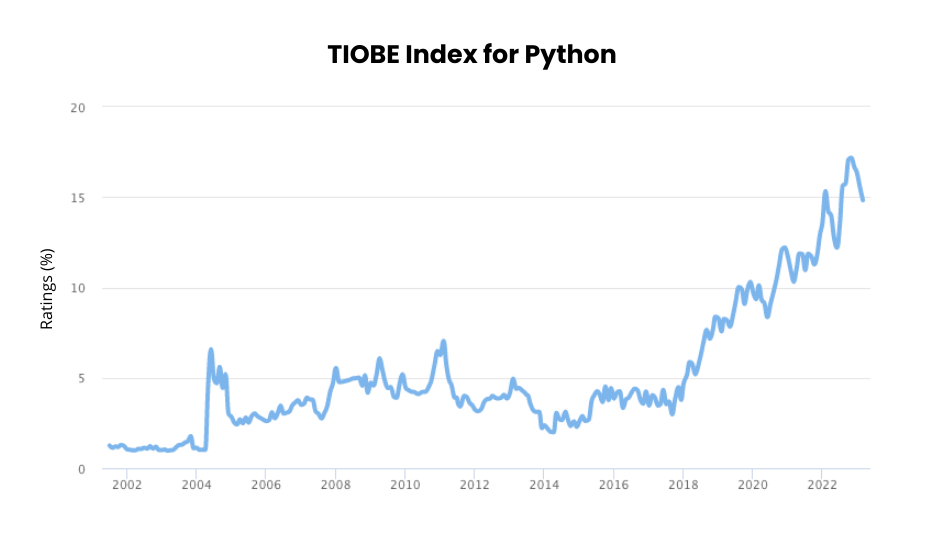
\includegraphics[width=\textwidth]{graphics/popularity}
\caption{Since the advent of Python 2.x, Python has yet to stop increasing popularity\\ \textbf{Source}: https://www.scalablepath.com/python/python-popularity}
\end{figure}

Before moving on, it's noted that since version 2.x, Python has engaged in "dual version release", which means that although 2.x may still receive various updates, the development team would also release version of Python 3.x. This became the status-quo since Python 2.6 released alongside Python 3.0. 


\subsection{Python in Today's World: Python 3.x}
In spite of the fact that Python 2.x was an explosive success, Python 3.x has been pushing Python to breaking the limits and constraints of the language itself. Thanks to the frequent and very active community, Python has constantly improved and added a wealth of features. \\
\hspace*{3mm} Released on December 3 2008\footnote{Python 3.0 - https://web.archive.org/web/20200614153714/https://www.python.org/download/releases/3.0/}, Python 3x (or "Python 3000" or "Py3k") ) was originally developed all the way back in the first Python 
\pagebreak

\section{Functional Programming}

\subsection{Lambda Calculus}

\hspace*{3mm} The backbone of Functional Programming is the art of Lambda Calculus. 	First introduced by mathematician Alonzo Church in the 1930s, Lambda Calculus is sometimes described as "the smallest universal programming language of the world"\footnote{Raúl Rojas - A Tutorial Introduction to Lambda Calculus}, for a good reason. It's a formal system of mathematical notations and modeling that assists in creating computer programs. Basically, instead using the old infix notations whenever we're discussing functions, lambda calculus equips us with a system of expressions and rules to make functions more readable and more logical, especially higher-order functions. To better comprehend this concept, we must understand how Alonzo Church defines a function. According to Church:

\begin{theorem}
\begin{verbatim}
function is a rule of correspondence by which when anything is given 
(as argument) another thing (the value of the function for that argument) 
may be obtained.
\end{verbatim}
\end{theorem}
\begin{figure}[ht]
\centering
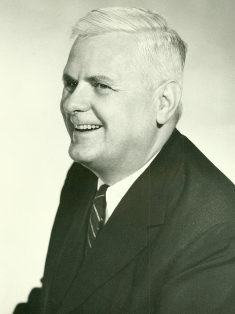
\includegraphics[width=0.35\textwidth]{graphics/church.jpeg}
\caption{Alonzo Church}
\end{figure}


This is a very primitive definition of a function, and Lambda Calculus (or $\lambda$ calculus) is essentially a family of notations that support representing functions as rules of correspondence. Consider the following example.\\
\hspace*{3mm} Let's say we write the function that takes in a single parameter $x$ and return the difference of $x$ and a constant value $y$. If we were to use the ordinary infix notation, we would get  $f(x) = x - y$ or you might write $f: x \rightarrow x - y$. This style of notation at first might seem intuitive and work out of the box, but let's consider an extension of the original function.]\\
\hspace*{3mm}Let's say we expand on the original $f$ function and equip it with a secondary parameter $z$. And, $z$ just so happens to be a function on its own: $z = g(y) = y+k$ with $k$ being a constant value. If we attempt to represent this function in the ordinary way, it would be very uncomfortable: $f(x,g(y)) = x - g(y) $. However, if we choose to use Church notations of $\lambda$ Calculus, things will get better.\\
\hspace*{3mm} First consider the original $f$ function, instead of writing it infix notation like before, we transform the secondary notation ($f: x \rightarrow x - y$) into a new one. We introduce the symbol '$\lambda$' for the parameter and write the function as: $f = \lambda x. x - y$. For each expression involving $x$, a notation for the corresponding function of $x$, we use the lambda expression. Now let's address the higher-order function, we simply rewrite as $(\lambda x \lambda y. x - (\lambda z. x + z)(y))$, the free variable introduced ($z$) is simply put into the inner function $g$.  Though it still seems clumsy, when applied in many more complex and higher-order functions, and especially when you program them, the $\lambda$ notation is substantially easier and more intuitive. It also provides us with a more systemic way of expressing functions. And always remember to use parentheses for your functions. \\
\hspace*{3mm} Here's a more formal structure for expressing $\lambda$ function:

\begin{center}

<function> := $\lambda$ <name> . <expression> 
\end{center}
\hspace*{3mm} The name after $\lambda$ is the identifier for the parameter, while the part after the dot is the expression or in programming we call "the body of the function". \\
\hspace*{3mm} There's a lot more about $\lambda$ Calculus to discuss about, but we're just going to go over substitution and focus on how this system of notations is applied into programming.

\subsubsection{Substitution}

\subsection{Functional Programming Paradigm}
\subsubsection{Definitions}
\hspace*{3mm} Functional Programming, at its core, is a new form of modeling problems. There are a plethora of definitions of Functional Programming. According to Professor Graham Hutton: "Functional Programming is a paradigm of programming in which methods of computation is the application of functions to arguments"\footnote{Graham Hutton}. In other words, a functional program is one that treats functions as the \textbf{first-class object}, the essential component of the program, and the entire structures of the program entirely relies on functions. Functions are like the blocks that make up the building which is the final program itself. From this definition of functional programming, it entails some aspects that distinguish it from other paradigms:

\begin{itemize}

\item Immutability
\item Functions are first-class object
\item Recursion
\item Pure Functions
\item Higher-order Functions
\item Curried Functions
\end{itemize}

\hspace*{3mm} These are some of the central aspects that a functional program must obey. A "Pure" Function is one that will always return the same value if the same parameter is passed onto the function. Thus, no side-effect is allowed, every time we repeat the same process of running a program (with the identical input), it's expected that it will always and always return the identical output.  This is one of the most vital reasons to why functional programming is so essential and valuable compared to other paradigms:the fact that we will only get what we expect will enhance debugging process, as side effects are out of the question, and the issue that a developer must address is the algorithm and logic, instead of minuscule and unpredictable elements.:
\begin{itemize}
\item Classes
\item Variable Declaration
\item Direct I/O streams
\item Iteration
\end{itemize}
 
\hspace*{1mm} Functional Programming also obeys a lot of other esoteric rules, but we leave these to be discussed in the sections on the application of this paradigm in Python. 

\subsubsection{Examples of Functional Programming Language: Haskell}

\hspace*{1mm} Though not very popular in industry, Haskell has become the poster child of FP, and has been one of the most fascinating languages in Academic Research. Developed in the late 2000s, Haskell is the embodiment of the ideas of FP. Every aspect of FP and Lambda Calculus is thoroughly integrated into the language itself. Consider a simple program that calculus the fibonacci sequence in Haskell: 

\begin{lstlisting}[language=Haskell, caption=Haskell Fibonacci]
fib 0 = 0
fib 1 = 1
fib n = fib (n-1) + fib (n-2)

\end{lstlisting}
\hspace*{1mm} This is very classic example of Haskell. Instead of inserting $\lambda$, we omit it and rewrite the structure into <function> <parameter> = <return value>, making it suitable for high-order functions. The code here leverages the recursive call, with the base case of the first 2 values of the Fibonacci sequence, and written according to the Haskell syntax we just mentioned.This implementation is very short, very concise and brief. For a non-programming person to take look at this snippet of code, they might even figure out what's the code does (assuming they do not know about the Fibonacci sequence that is!). The syntax feels like typical Math expressions, which is one of the key characteristics of FP languages and modules in general-purpose languages. 
\subsubsection{The Advantages of Functional Programming}
\begin{itemize}
\item Ease of debugging: Since the infrastructure of our code is based entirely on functions, and we avoid as much side effects as possible, it's much less cumbersome to find issues and bugs in your program. As functions are pure and variables can be isolated from various control flow.
\item Less abstraction: One of the major problems modern developers have with OOP is how some people overuse it and make their code impractical and unreadable. With functional programming, abstraction is stripped down and limited to a very minimal amount, just enough for future maintenance.
\item Simpler Code: With the lack of loops, conditions, methods,... the code is much shorter and less dense.
 

\end{itemize}

\hspace*{1mm} Aside from these 3 central advantages of functional programming, learning and mastering the crafts of Functional Programming can help developers leverage their mathematical modeling skill and better design programs, regardless of paradigm. Modern languages which have comprehensive functional features would be a massive benefit for coding, since those features allow us to combine OOP with FP, getting the best of both world. And Python is (arguably) the best general-purpose language that features a comprehensive functional libraries and modules. The next section will be an introduction to basic Python, so that we can dissect and investigate the FP patterns in Python.

\section{Basic Programming and Functions in Python}
\subsection{The Basic Elements}
\subsubsection{Creating a Python file}
\hspace*{1mm} A Python program has file extension ".py", which stands for Python obviously. However, were you to use Python as a scripting notebook (as Rossum intended), you should use the extension ".ipynb" to create a script of Python, instead of a full Python program.\\
\hspace*{6.5mm} First and foremost, we need to install the Python Interpreter. Unlike C++ and C, there aren't various compilers for the language, since Python is developed by the Python Software Foundation\footnote{The Python Software Foundation - https://www.python.org/psf-landing/}. The Interpreter downloaded from https://www.python.org can be run without much issues on every supported operating system, like how JVM is "Write Once, Run Everywhere"\footnote{What is Java? - https://www.ibm.com/topics/java}. This is another reason Python is so accessible: No need to worry about the complexity of installation, like that of C++/C or some older languages. We'll not going into the details installation, since each operating system has its own way of installing Python, but generally the Python official site should give you the correct instructions.\\
\hspace*{6.5mm} Once we've got Python up and running, we can create a .py (or .ipynb) file to run Python. In this report, to simplify things we'll demonstrate Python through a .py file, since it help us with running a complete function program in the implementation section. We'll also use VsCode to demonstrate the Python source code, however note that Python has a plethora of IDEs and Text Editor, just pick the one you're most comfortable with\footnote{Python IDEs and Code Editors (Guide)- https://realpython.com/python-ides-code-editors-guide/}.
\begin{figure}[ht]
\centering
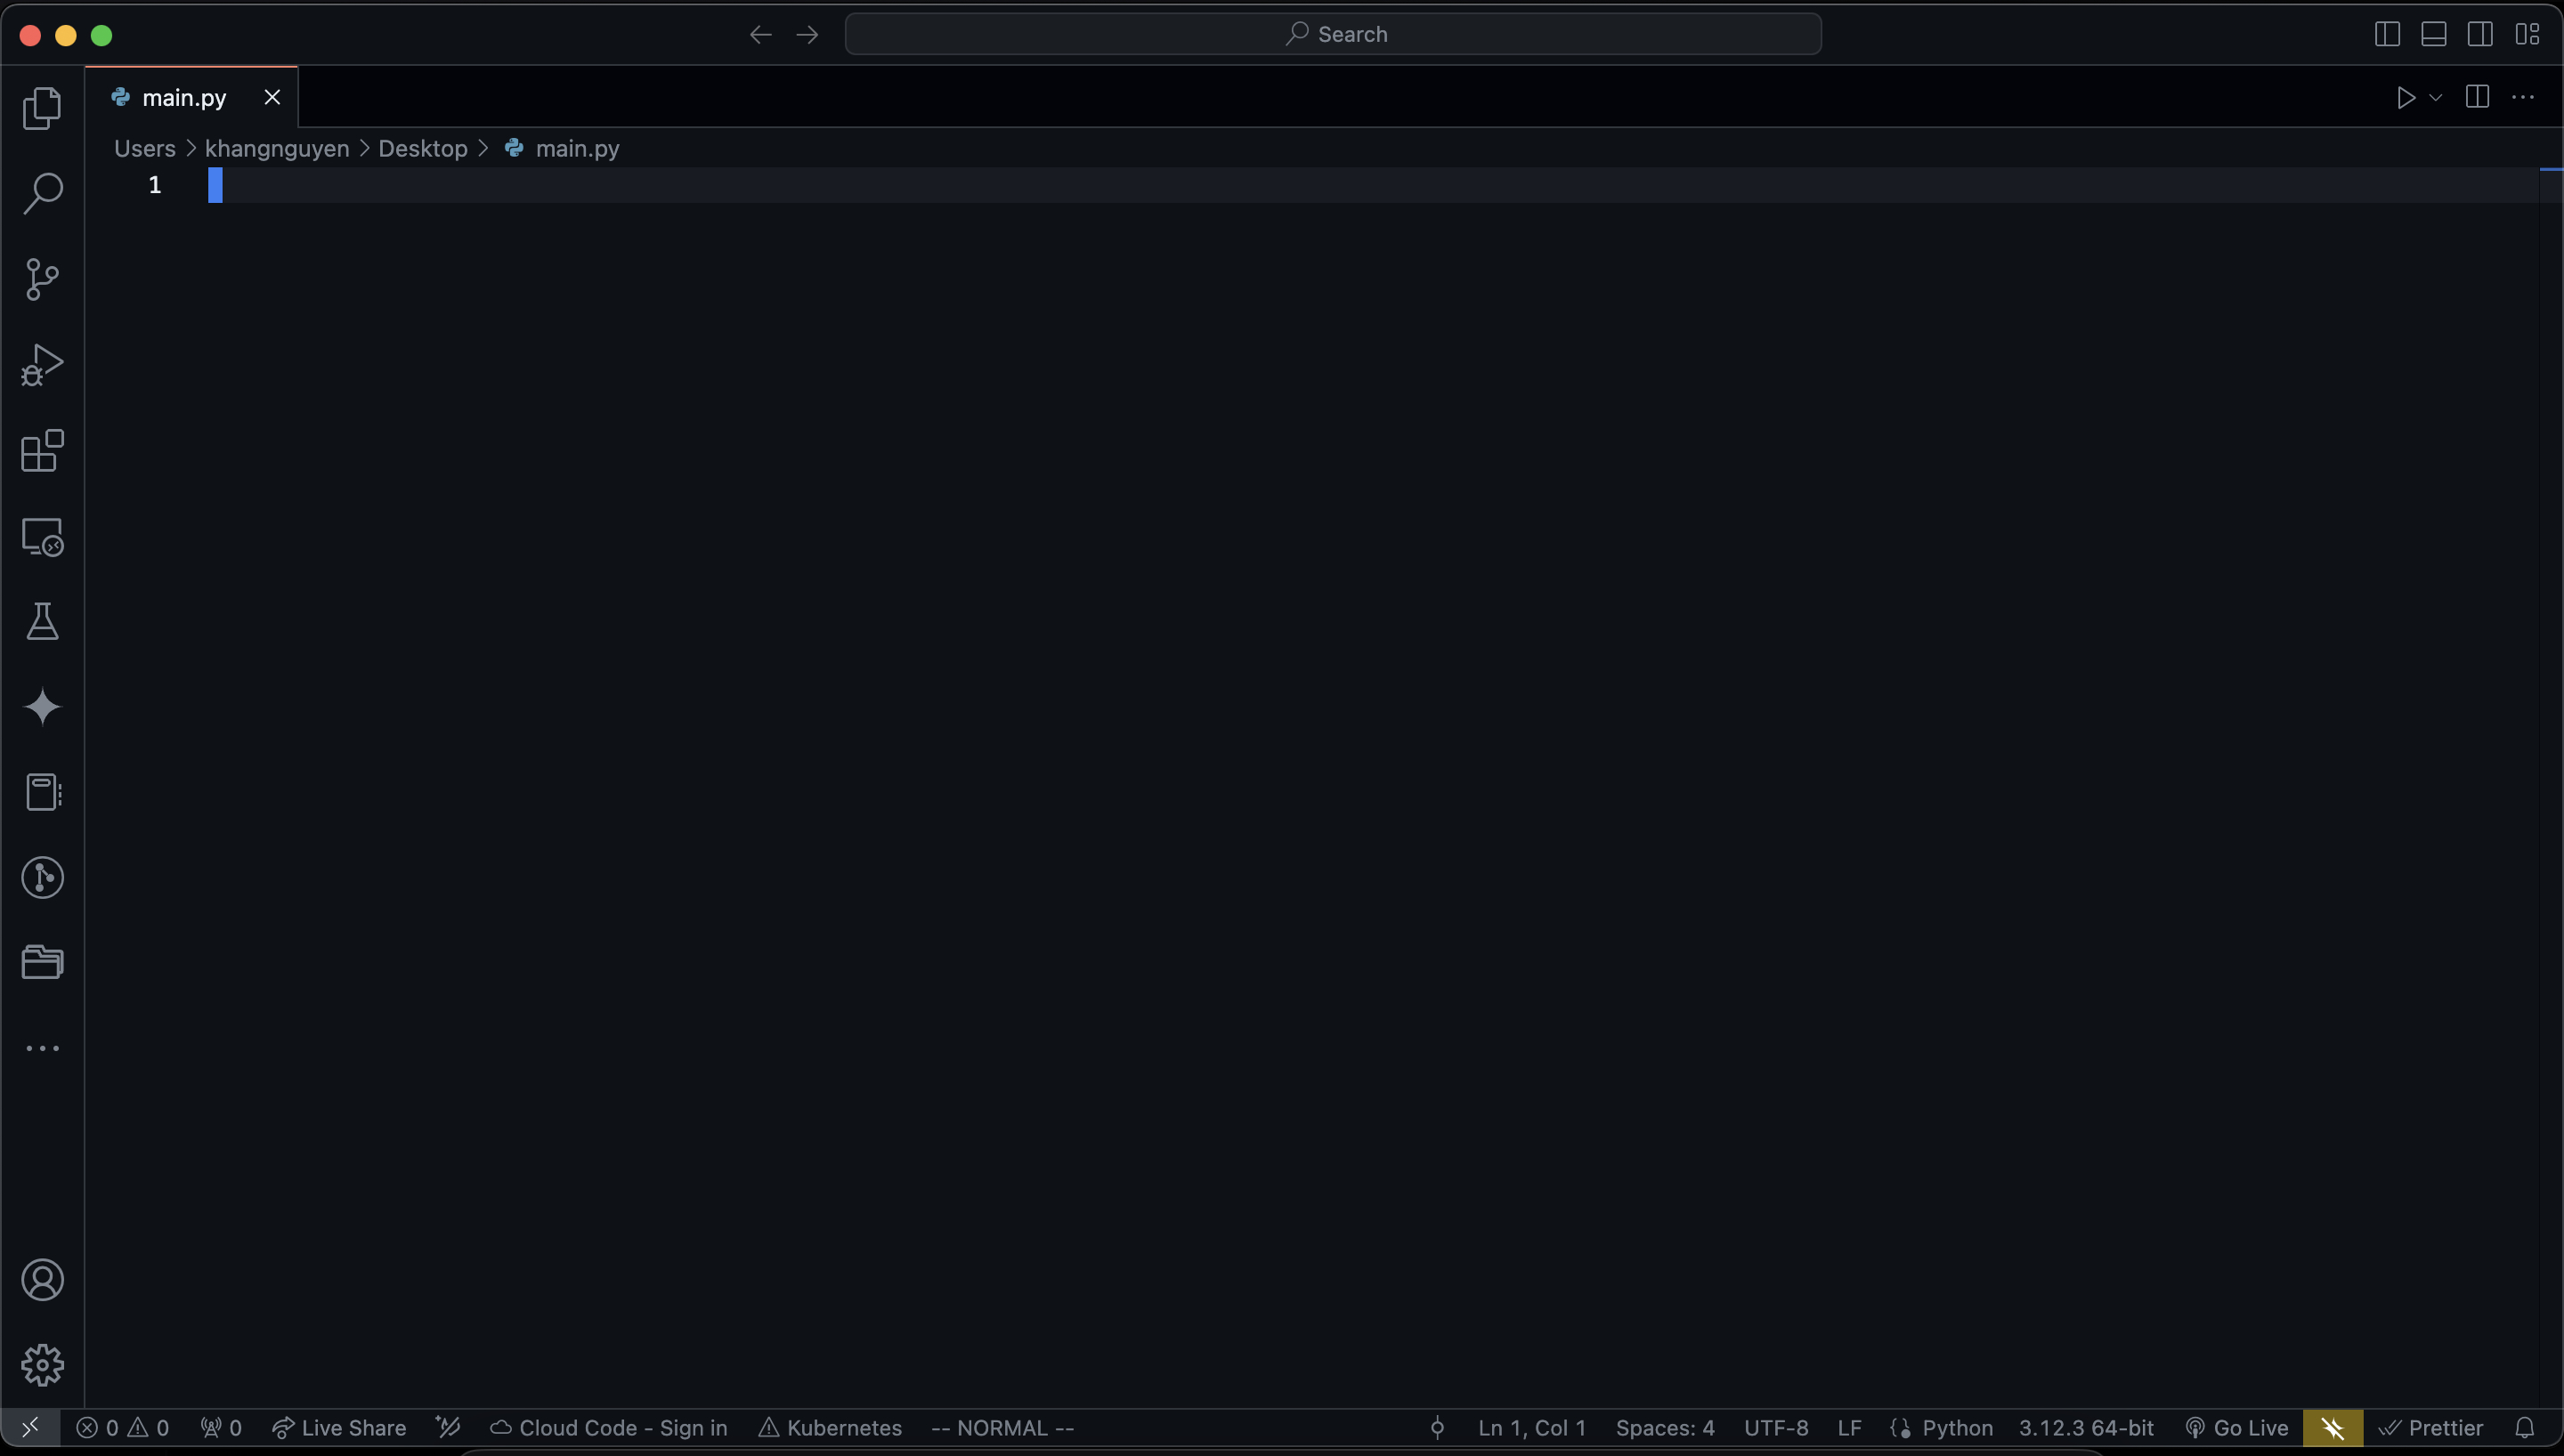
\includegraphics[width=\textwidth]{graphics/python1}
\caption{A Fresh Python setup on VsCode (MacOS)}
\end{figure}
\pagebreak

\subsubsection{Types in Python}
\hspace*{1mm} If you're a C++,C,Fortran or Java developer, you would be astonished by Python elegant and simple syntax. Like we've said, Python is dynamically-typed, so we needn't specify the type of our variable and objects. Let's say we want an integer \textbf{$x$} with the value 4, we simply type: $x = 4$. The interpreter will deduce what type x is (integer) in runtime. It's worth noting the various types that Python offers. The complete inventory of Python built-in types includes:
\begin{itemize}
\item Integer and floating points objects
\item Complex number objects
\item Decimal: fixed-precision objects
\item Fraction: rational number objects
\item Sets: collections with numeric operations
\item Sequence Types: List, Tuples, Dictionaries,...
\item String types
\item Booleans: true and false
\end{itemize}
\hspace*{6.5mm} Please be aware that this list does not include the types in various Python external libraries. We can use the $type()$ function to get our type. Our above expression $a = 3 $ will be deduced as type 'int'. Observe the following output: 
\begin{figure}[ht]
\centering
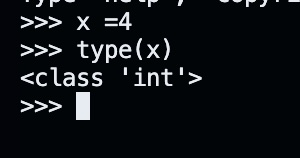
\includegraphics[width=0.3\textwidth]{graphics/python2}
\end{figure}
\begin{center}
\begin{verbatim}
Why is it "class 'int'"?
\end{verbatim}
\end{center}
\hspace*{6.5mm} In Python, everything is treated as an "object", a piece of memory that may contain values or set of associated operations. The reason for this is because Python is dynamically typed, type of a variable or function can't be assigned before runtime. Thus, the interpreter just allocate an area of memory, called object, first (may not be fixed before runtime), then when the program reaches that part of the code containing the object, it will do its work and deduce the suitable type for the object. Thus, Python considers each of its built-in types to be a "class". "Class" here simply means a kind of object, or a "type" of object, like the concept of class in OOP, since every variable, function is an object. That's why we call it "class 'int' ", not "type 'int'".\\
\hspace*{6.5mm} Moreover, Python, at runtime, links the variable declared in the code to the corresponding object, using a reference, like a link or association of a variable to an object. One thing to remember that distinguishes Python from C/C++ is that pointer does not exist in Python, they're the "reference", due to the fact that Python takes care of all the dynamic memory allocation for us. To simplify all the terminology we just discussed:
\begin{itemize}
\item \textbf{Variables} are entries in symbol table, with space for links to object.
\item \textbf{Objects} are jut pieces are allocated memory (by the interpreter) to represent the suitable type for the variable.
\item \textbf{Reference} are automatically followed pointers (or links) from the variables to objects.
\end{itemize}
\begin{figure}[ht]
\centering
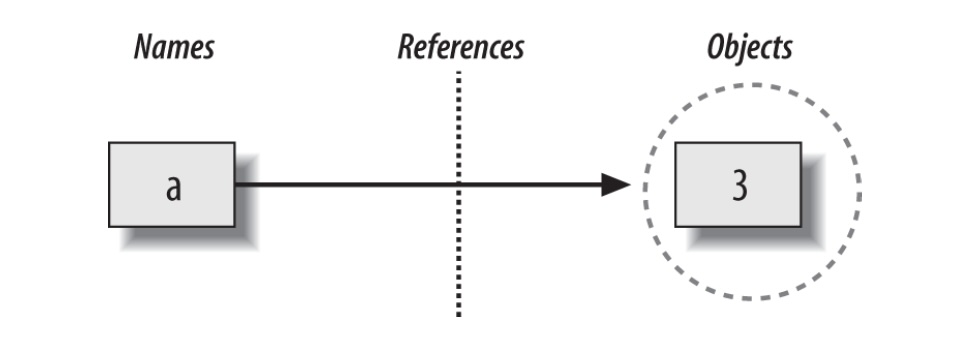
\includegraphics[width=0.9\textwidth]{graphics/python3}
\caption{How Python maps variable to its object}
\end{figure}
\hspace*{6.5mm} This concept of object will be central to understand how Python works under the hood, and gives us more insight to how to create effective fluent Pythonic programs.\\
\hspace*{6.5mm} Getting back to syntax, aside from simple numeric types, we can also assign with strings: 


\begin{lstlisting}[language=Python, caption=A Few Examples of Assignment in Python]
a = 23 	#numeric assignment (int)
str = " Hello World" #string assignment
b = 12.34 #numeric assignment (float)
c =  (2<3) #boolean value (bool)
\end{lstlisting}
\hspace*{6.5mm} These types and syntax our the basic building blocks to progress further in Python. Now, we need to expand to another domain of Python types, which is garbage-collection and memory safety.
\subsubsection{Garbage Collection}

\subsubsection{Operations on simple types}
\hspace*{1mm} In Python, we need not worry about getting our memory "leaked". The interpreter, after the program has terminated, 
\subsubsection{Immutability}
\hspace*{1mm} In C++, we're accustomed to types being fully modifiable, or mutable, unless they're \textbf{const} value. This is absolutely not the case in Python. \\
\hspace*{6.5mm} Some data types are mutable (the numeric types), but some cannot be modified and are thus immutable (string, tuples,...). \\
\hspace*{6.5mm} Let's take string for example. If I have a string $str$, if I initialize it as "Hello", next time I assign it to "World", it does not overwrite the original object ("Hello"). Rather, it just changes its reference, and points to a newly allocated object "World". However, if I want to change the first character 'H' to 'W', getting "Wello", it's illegal since I'm modifying an immutable type. Observe the below example:\\
\begin{figure}[ht]
\centering
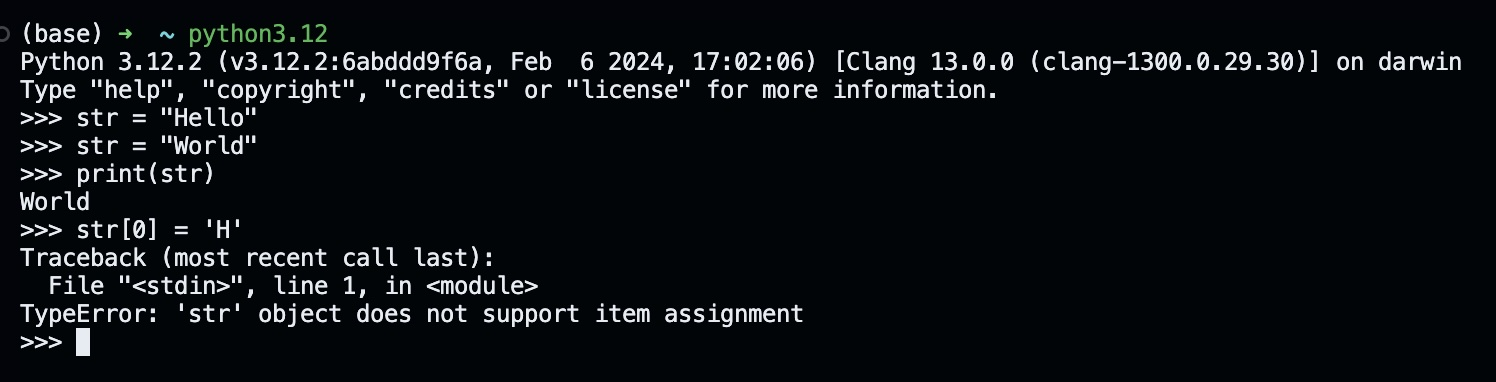
\includegraphics[width=0.9\textwidth]{graphics/python4}
\caption{Mutability of string}
\end{figure}
\hspace*{6.5mm} Mutability also applies to several other data types in Python. Immutability is essential in Functional Programming, because it helps us prevents side effects, thus preserving the core ideas of FP.\\
\hspace*{6.5mm} It's noted that Python (standard library) provides a huge library of built-in methods, like we've demonstrated print() and type(). These would come into good use when we discuss FP in Python. And speaking of functions. The next section will be about how we create functions, just ordinary functions in Python. This is key in understanding more abstract concepts about FP in Python later on.


\subsection{Functions in Python}
\hspace*{1mm} Before diving into the colorful FP features of Python, we need to go through how is it a function works in Python. From this foundational knowledge on functions, we can better utilize FP in Python.
\subsubsection{The def keyword}
\hspace*{1mm} To declare a function, we need the \textbf{def} keyword. The structure is as follows:
\begin{verbatim}
	def <function name>:
			(indentation) <function body>
\end{verbatim}
\hspace*{6.5mm} Unlike in complied langues, since we uses dynamic typing, we do not declare the return type of the function. We just need def to specifies that we're declaring a functions. Just like variables, def creates an object in memory (done by the interpreter) and assign the function name to that object. The function name then becomes a reference for that object. If the function contains attributes in it, the memory space for those attributes are also included in the object. \\
\hspace*{6.5mm} In the <function name>, we must also include the  (), even if our function has no parameters. \\
\hspace*{6.5mm} Our functions can also be "void", it can just do some operations yet returns none, just don't include the \textbf{return} line.  When a function is called, the caller (usually the process) halts its execution of that piece of program and lets the function does its work until it finishes or stops and returns the control back to the caller, just like with other languages.\\
\hspace*{6.5mm} There are a lot of aspects about functions that we need to note, which we'll discuss now. Firstly, let's cover the calls of a function.
\subsubsection{Function Calls}
\hspace*{1mm} A function can be defined anywhere in the program, but only when it's actually called that Python initiate an instance of the function. The function code is a passive entity, while the function call itself is an active entity. Take a look at the below example:

\begin{lstlisting}[language=Python, caption=Simple Summation Function]
def sum(a,b):
    return a + b #function declared here

print(sum(12,23)) #function call
print(sum(12.2,22.2))		#function call

\end{lstlisting}

\hspace*{6.5mm} As you can see, the $sum(a,b)$ function is declared from line 1 to 2, but it's only called later on. This function can be used for both integers and floats, which is an aspect of function named \textbf{polymorphism}, which we'll discuss later. We must remember that you can only call a function when it's has already been declare. Since Python has no function prototype, we must fully defined it before the calls.
\begin{lstlisting}[language=Python, caption=Function call before definition]
area(1,2)
def area(x,y):
    return x*y
area(45,23)
\end{lstlisting}
\hspace*{6.5mm} From the code above, the program will not able to calculate, since the $area(x,y)$ function was not avail at the $area(1,2)$ call, so the $area(x,y)$ is just undefined behaviors. Before moving on, let's have a look at another example:
\begin{lstlisting}[language=Python, caption=Execute until error]
print("The Area")
area(1,2)
def area(x,y):
    return x*y
area(45,23)
\end{lstlisting}
\hspace*{6.5mm} If we run the above code, the program would still prints "The Area", since Python is an Interpreted Language, it will compile and run each line, then proceed with the next line. That may explain why function call before function definition does not work, the interpreter has not reached the definition yet!\\
\hspace*{6.5mm} Going back to the Listing 5.2, let's investigate the polymorphism to talked about before. 
\subsubsection{Polymorphism}
\hspace*{1mm} In OOP, polymorphism refers to an abstract class (with only the definitions) with multiple concrete implementation. In Python (and many FP languages), Polymorphism refers to a function that can take in and produces multiple data types. From Listing 5.2, we saw that the summation function can take and return both floats and integers. Thanks to Dynamic Typing, the function's real return type isn't defined before runtime, thus only when it's called that the type is deduced.  So the function can "morph" into many forms, taking and returning various different types. If the interpreter cannot find a suitable type, it will return an error call.
\\ \hspace*{6.5mm}This is one of the most crucial philosophical differences between Python and statically typed languages like C++ and Java: in Python, your code is not supposed to care about specific data types. The polymorphism feature helps a lot, especially when you're using Python for scripting, you only need to care about the operations of the function, no need to create multiple version of the function with diverse types, this is exactly what Guido Van Rossum wanted. We will revisit Polymorphism when we get into FP in Python, since this is a very important featue. 
\subsubsection{Scope of Variables}
\hspace*{1mm} Just like how function calls can be executed when the interpreter reaches them, variables and functions can only be used when the interpreter has reached them. Moreover, the local variables can only be declared in be available in its local scope. For functions:
\begin{itemize}

\item Names assigned inside a def can only be seen by the code within that def (alignment level). The name can't be referred outside of that def scope.
\item Names assigned inside a def cannot be conflicted with variables outside the def.
\item If a variable is assigned in a def, it's local to that def.
\item If a variable is assigned in an enclosing def, it is nonlocal to nested functions.
\item If a variable is assigned outside all defs, it is global to the entire file.
\item Each time you create a new function call, a new function scope is created.
\end{itemize}
\hspace*{6.5mm} Have a look at the below code snippet: 
\begin{lstlisting}[language=Python, caption=Scope Variable Error]
x = 12
def foo(n,k):
    l = 233
    return (l*k**n)
print(x)
print(l)
\end{lstlisting}
\hspace*{6.5mm} Here x is a global variable, thus every def, every inner scope can access (and modify in this case) the variable $x$. However, $l$ itself is local to the function $foo(n,k)$ can thus cannot be accessed outside of the function scope. Have a look at another example:
\begin{lstlisting}[language=Python, caption=Another Scope Variable Error]
def foo1(n,k):
    q = 74
    return(n**k*q)
x = 123

def foo2():
    return x**5 

def foo3(e):
    return q*e
\end{lstlisting}

\hspace*{6.5mm} Here, $x$ is a global variable so any def or structures can access that variable. q is local to the function $foo1(n,k)$, and cannot be accessed by $foo3(e)$ here, which will make Python give an error.\\
\hspace*{6.5mm} One very popular rule that the Pythonistas often use is the LEGB rule for variable scope. Each of these letters stands for: Local, Enclosing, Global, Built-in scope:
\begin{itemize}
\item Local scope: the code block or body of any Python function.
\item Enclosing Scope: a special scope that only exists for nested (composite) functions.
\item Global scope: the top-most scope in a Python program, script, or module, visible to all functions and modules in a file.
\item Built-in scope: a special Python scope that’s created or loaded whenever you run a script or open an interactive session

\end{itemize}
\hspace*{6.5mm} This is a pretty useful cheat sheet for Python beginner. The first 3 ones are familiar, a "built-in scope" is one that 

\hspace*{6.5mm} Another idea for scope in Python, is about Composite Functions, which directly relates to why ordinary functions may not be the best choice.\\
\subsubsection{Composite Function}
\hspace*{6.5mm} Just like other functions, you can define a new function inside your function, or an "inner function". Every attributes of the inner function is also local to that inner function only, and thus cannot be accessed by the outer function, or other functions. Have a look at the following example:
\begin{lstlisting}[language=Python, caption=Composite Function]
def foo2():
    def foo21():
        t = 87
        return t**t
    e = foo21()%(foo21()/t)
    return foo21()**5*e

print(foo2())

\end{lstlisting}
\hspace*{6.5mm} From the example code above, it can be seen that $foo21()$ is a inner function of $foo2()$, and thus if any other function attempts to access variables inside foo21(), it's not possible (which is t in this case). Not even foo2() can access $t$, the above code snippet will give us an error and does not execute properly. One can inferred from the above code: It's too cumbersome to write a nested function like this. Since $foo21()$ is going to be used only by $foo2()$ anyway, it's a disposable function. Let's have a look at another example: we implement a function that emulates a calculator, but using only functions: 
\begin{lstlisting}[language=Python, caption=Composite Calculator Implementation]
#nested function calculator function with all the operators
def calculator(a, b, operator):
    def add(a, b):
        return a + b
    
    def subtract(a, b):
        return a - b
    
    def multiply(a, b):
        return a * b

    def divide(a, b):
        if b != 0:
            return a / b
        else:
            return "Error: Division by zero"
    if operator == "+":
        return add(a, b)
    elif operator == "-":
        return subtract(a, b)
    elif operator == "*":
        return multiply(a, b)
    elif operator == "/":
        return divide(a, b)
    else:
        return "Error: Invalid operator"
\end{lstlisting}
\hspace*{6.5mm} Using nested functions like this, it creates a layer of encapsulation and protects our disposable methods. Though this is very laborious and cumbersome, and the code pretty much "smells". You can use class in Python to somewhat alleviate this, but it's no better. A way to fix this effectively, is using a lambda functions:
\begin{lstlisting}[language=Python, caption=Composite Calculator Implementation]
def calculator(a, b, operator):
    add = lambda a, b: a + b
    subtract = lambda a, b: a - b
    multiply = lambda a, b: a * b
    divide = lambda a, b: a / b if b != 0 else "Error: Division by zero"
    return {
        "+": add(a, b),
        "-": subtract(a, b),
        "*": multiply(a, b),
        "/": divide(a, b)
    }.get(operator, "Error: Invalid operator")
    \end{lstlisting}
\hspace*{6.5mm} We may not understand most syntax in this yet, but leveraging FP in Python really does help us with reducing code complexity and make it so much simpler. This is why we invest so much time into learning FP, it make our code so much better looking and refactorable. This wonderful aspect of Python will be thoroughly dissected in the next sections.
\subsubsection{Argument Passing}
\hspace*{1mm} One major departure from C++ and Java that Python takes is how it deals with argument passing. A C++ developer is used to pass-by value, pass-by reference and pass-by pointer, which differ in how they modify the original value or create a copy to passed to a function. Python, however, has a very interesting and dissimilar mechanism for passing parameters. \\
\hspace*{6.5mm} Firstly, remember that variables in Python are \textbf{objects} that are type-deduced at runtime. Thus, the way in which we refer to passing in Python is a complete an new form called "pass-by assigment", or some may call pass-by-object-reference, but we'll stick with the former for brevity. This essentially means passing our object to the parameters of the functions, which are just variables (and as we later discussed, could be functions).\\
\hspace*{6.5mm} Since types are deduced in runtime, we does not have complete control over the passing mechanism. In C++, we can easily decide if it's pass-by value or reference or pointer by just declaring the formal parameter:
\begin{lstlisting}[language=C++, caption=The 3 different Argument-Passing Mechanism in C++\\ We can decide which one is suitable for our function]
int foo1(int a)
{
    a +=2;
    return a;
}
int foo2(int* a)
{
    *a += 2;
    return *a;
}

int foo3(int &a)
{
    a += 2;
    return a;
}
    \end{lstlisting}
\hspace*{6.5mm} The same can't be said about Python, it always defaults to pass-by-object. So what's pass-by object specifically?\\
\hspace*{6.5mm} Pass-by-object combine the mechanisms of pass-by-value and pass-by-reference. When a function is invoked, each identifiers in the formal parameters are assigned the value of the actual parameters, according to the principle of assignment. Recall how assignment works in Python: a variable is assigned to an object in memory through a reference.
\pagebreak
\bibliographystyle{plain}
\bibliography{refs/example.bib}
\nocite{*}

\end{document}
